
\begin{figure}[!ht]
    \centering


\resizebox {0.9\columnwidth} {!} {
     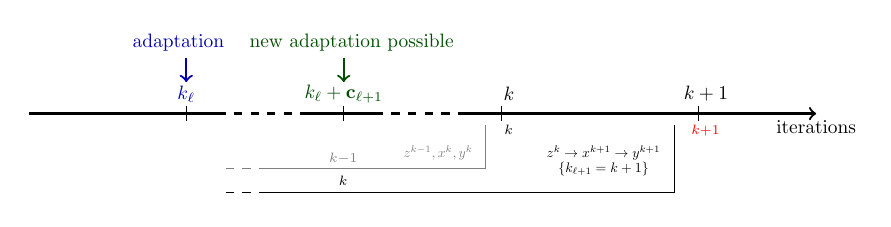
\begin{tikzpicture}
     %%% BASE
    \draw[thick, ->] (0,0) -- (10,0) node [below,scale=0.7] {iterations};
    \foreach \x in {1,...,3}
    \draw (2*\x, 0.1) -- node[pos=0.5] (point\x) {} (2*\x, -0.1);
    \draw (8.5, 0.1) -- node[pos=0.5] (point4) {} (8.5, -0.1);
    
    
     
          \draw[thick,dashed,white] (2.5,0) -- (3.5,0);
          \draw[thick,dashed,white] (4.5,0) -- (5.5,0);
    
    \node[scale=0.7] at (2,0.25) {\color{blue!70!black} $k_\ell$};
    

    \draw[thick,blue!70!black, ->] (2,0.7) -- (2,0.4) ;
    \node[scale = 0.7] at (1.9,0.9) {\color{blue!70!black} adaptation};
    
    

    
    
    
            %%% COord
            

    
   % \draw[thick,green!70!black, ->] (3,0.5) -- (3,0.1) ;
%    \node[scale = 0.7] at (3,0.7) {\color{green!70!black} coordination};
    
        \draw[thick,green!30!black, ->] (4,0.7) -- (4,0.4) ;
    \node[scale = 0.7] at (4,0.25) {\color{green!30!black} $k_\ell + \mathbf{c}_{\ell+1}$};
        \node[scale = 0.7] at (4.1,0.9) {\color{green!30!black} new adaptation possible};
    
    
    \node[scale = 0.5, gray] at (5.2,-0.5) { $z^{k-1},x^{k},y^{k}$};
    
    \node[scale = 0.7] at (6.1,0.25) { $k$};
    \node[scale = 0.7] at (6.1,-0.25) { $\Sel^k$};

    \draw[gray] (5.8,-0.15) -- (5.8,-0.7) -- (3,-0.7);
    \draw[dashed,gray] (2.5,-0.7) -- (3,-0.7);
    \node[scale = 0.7,gray] at (4,-0.6) { $\FF^{k-1}$};

    
    \node[scale = 0.5] at (7.3,-0.5) { $z^k\to x^{k+1} \to y^{k+1}$};
    \node[scale = 0.5] at (7.3,-0.7) { $\{ k_{\ell+1} = {k+1}\}$};
    
    \draw (8.2,-0.15) -- (8.2,-1.0) -- (3,-1.0);
    \draw[dashed] (2.5,-1.0) -- (3,-1.0);
    \node[scale = 0.7] at (4,-0.9) { $\FF^{k}$};
    
    
    \node[scale = 0.7] at (8.6,0.25) { $k+1$};
    \node[scale = 0.7,red] at (8.6,-0.25) { $\Sel^{k+1}$};



    
  %  \draw [very thick,green!70!black,->] (3,-0.1) to [out=-30,in=-150] (4.5,-0.1) ;
   %  \node[scale = 0.7] at (3.75,-0.5) {\color{green!70!black} $\leq T$};    
    
    %\draw [very thick,green!30!black,->] (4.5,-0.1) to [out=-30,in=-150] (6.5,-0.1) ;
    % \node[scale = 0.7] at (5.5,-0.5) {\color{green!30!black} $\leq T'$};
    
    
  \end{tikzpicture}}
  
  
      \caption{Summary of notations about iteration, adaptation and filtration. The filtration $\mathcal{F}^{k-1}$ is the sigma-algebra generated by $\{\Sel^\ell\}_{\ell\leq k-1}$ encompassing the knowledge of all variables up to $y^k$ (but not $z^k$).}
    \label{fig:proof}
  
  \end{figure}
